\subsection{List des compétences}
Vous trouverez ici les Compétences utilisables dans \swr. L’utilisation d’une Compétence en situation normale ne devrait pas donner lieu à un jet de dé. Seules les situations de stress, lorsque le temps est compté ou que la réussite est loin d’être acquise, devraient donner lieu à un test de Compétence.

On trouve entre parenthèses l’attribut associé à la compétence.

\begin{description}[align=left]
    \item [Combat (Agi)]
        Combat englobe toutes les attaques de corps à corps quelle que soit l’arme de mêlée utilisée.

    \item [Conduite (Agi)]
        Conduite permet à votre héros de conduire les véhicules terrestres ou aéroglisseurs courants de l’univers Star Wars.

    \item [Connaissance (Int)]
        Connaissance est une Compétence passe-partout qu’il faut spécialiser. Elle inclue aussi les langues autre que la langue natale et le Basic. Par exemple on peut utiliser les spécialisations suivante : Force, Jedi, Sith, Aéronautique, Informatique, Bataille, \ldots Dans tous les cas, on parle de connaissances théoriques et non pratiques.

    \item [Discrétion (Agi)]
        Discrétion représente la faculté à se cacher et à se déplacer en silence, mais aussi de camoufler des objets ou de subtiliser de petits objets à l’insu de tous.

    \item [\'Equitation (Agi)]
        \'Equitation permet de monter, contrôler et chevaucher tout animal domestiqué.

    \item [Escalade (For)]
        Les personnages peuvent être amenés à escalader des obstacles ou grimper une falaise pour prendre l’avantage du terrain lors d’une attaque, ou encore pour échapper à un ennemi trop coriace.

    \item [Intimidation (\^Ame)]
        Intimidation est l’art d’effrayer un adversaire par la force de sa volonté, que ce soit par une menace ouverte ou voilée ou tout simplement avec un énorme flingue.

    \item [Jeu (Int)]
        Voici un moyen rapide pour simuler une demi-heure d’une partie de jeu sans lancer les dés pour la moindre phase du jeu en question.

    \item [Lancer (Agi)]
        Lancer s’applique à toutes les armes qui se lancent, grenades, couteaux, haches, lances, etc.

    \item [Natation (Agi)]
        Natation détermine si un personnage nage ou coule comme une pierre lorsqu’il se trouve dans l’eau, ainsi que sa vitesse de déplacement en milieu aquatique.

    \item [Navigation (Int)]
        Navigation est la capacité du personnage à voyager et à se repérer dans l’espace. Il englobe aussi l’entretien journalier de l’équipement utilisé.

    \item [Maîtrise de la Force (\^Ame)]
        C’est la compétence qui mesure le niveau de votre héros à l’utilisation de la Force. Cette compétence ne sert à rien sans l’Atout Arcane (Force).

    \item [Perception (Int)]
        Perception représente la vigilance d’un héros et son habileté à découvrir objets ou indices.

    \item [Persuasion (\^Ame)]
        Persuasion représente la capacité d’un héros à convaincre les gens qu’il rencontre. Même s’il ne le fait pas délibérément, la Force vient souvent appuyer les facultés de persuasion.

    \item [Pilotage (Agi)]
        Pilotage permet d’utiliser tous les types d’appareils aériens ou spatiaux communs.

    \item [Piratage (Int)]
        Cette compétence permet à celui qui la possède de pirater les systèmes électroniques comme les serrures ou les systèmes de contrôle dans un vaisseau ou un base.

    \item [Pistage (Int)]
        Pistage permet de suivre les traces d’un ou de plusieurs individus sur tout type de terrain.

    \item [Recherche (Int)]
        Recherche permet d’obtenir des informations dans une bibliothèque, sur l’HoloNet, dans les journaux ou toute autre source écrite.

    \item [Réparation (Int)]
        Réparation représente la capacité à remettre en état gadgets, véhicules, armes et autres machines.

    \item [Réseaux (Int)]
        Réseaux permet d’obtenir des informations dans la rue, les bars ou par des contacts en utilisant la menace, la corruption ou en offrant des verres. Cette compétence peut aussi représenter les informateurs du héros.

    \item [Sarcasme (Int)]
        Sarcasme est une attaque contre l’amour-propre d’un individu en le ridiculisant par la parole ou le geste.

    \item [Soins (Int)]
        Soins consiste à savoir comment guérir les plaies et traiter les blessures.

    \item [Survie (Int)]
        Survie permet de trouver nourriture, eau ou abri en milieu hostile.

    \item [Tir (Agi)]
        Tir concerne toute tentative pour toucher une cible avec n’importe quelle arme à distance (arc, pistolet, lance-roquettes, etc\ldots).
\end{description}
\clearpage
\begin{paperbox}{Navigation}
    La navigation existe mais son domaine d’application change un peu, on ne parle pas dans Star Wars de bateau mais de vaisseaux spatiaux. La navigation est alors la capacité du héro à s’orienter dans le vide sidéral. Mais cela s’applique aussi au sol pour se repérer sur une carte par exemple.
\end{paperbox}

\vspace*{\fill}
\hspace*{-0.5\columnsep}
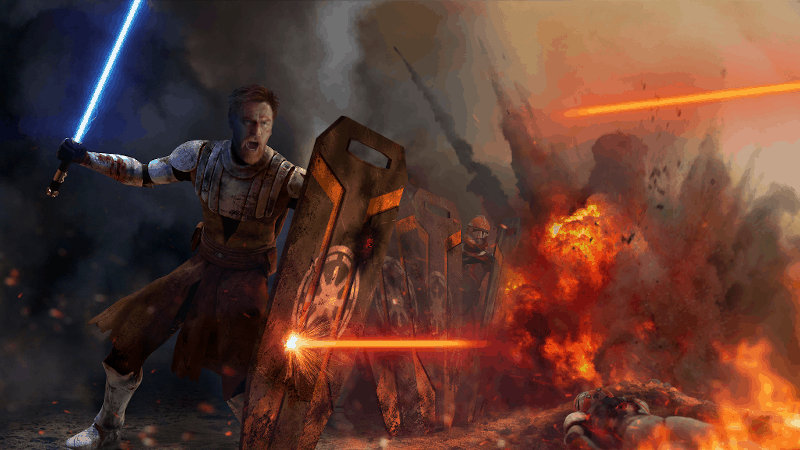
\includegraphics[width=\textwidth]{img/personnages/skills.jpg}

\newpage
\begin{paperbox}{Piratage}
    Cette compétence vient remplacer le Crochetage qui dans Star Wars n’a pas une grosse utilité. La compétence Piratage (Informatique) va s’utiliser de la même façon mais sur l’Intellect au lieu de l’Agilité. L’informatique pourra être utilisé dès qu’un ordinateur entre en scène. On pourra par exemple déverrouiller des sas de vaisseau, stopper un signal d’alarme ou encore désactiver des capteurs à plus haut niveau.

    Les Droïdes n’en sont pas systématiquement pourvu, cela dépend de leur programmation.
\end{paperbox}
